\section{\textit{b}-flow}
\textit{Find for each of the two graphs in Figure \ref{fig:bflow}, a b-flow for the graph or argue that the graph has no b-flow}
\begin{figure}[h]
  \centering
  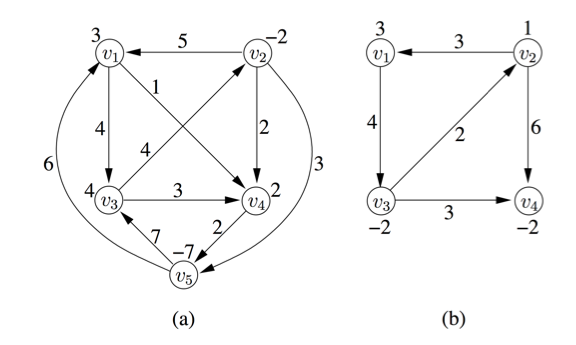
\includegraphics[scale=0.4]{images/bflow_graphs.png}
  \label{fig:bflow}
\end{figure}

For a directed graph \(G=(V,E)\). For each vertex \(v \in V\) let \(\delta^+(v)\) be the set of outgiong edges from \(v\) and \(\delta^-(v)\) be the set of incoming edges to \(v\).\\
Given is that each a \textit{b}-flow under the following constraints
\begin{align}
  \sum_{e\in \delta^-(v)} x_e - \sum_{e\in \delta^+(v)} x_e =&\, b_v, \forall v \in V\label{eqn:const1}\\
  0 \leq x_e \leq&\, u_e, \forall e \in E\label{eqn:const2}
\end{align}

\noindent Given these constraints we find that the following \textit{b}-flows exist for graph (a)
\begin{align*}
  \delta (v_2v_4) =&\, 2\\
  \delta (v_5v_3) =&\, 4\\
  \delta (v_5v_1) =&\, 3
\end{align*}

\begin{figure}[ht]
  \centering
  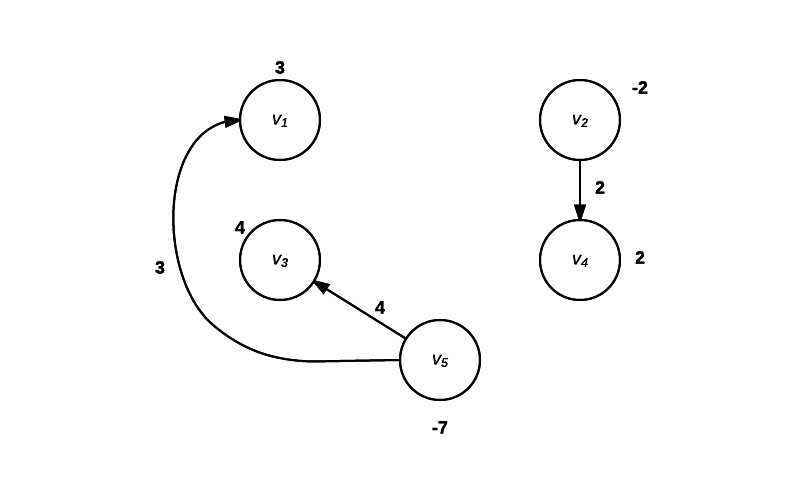
\includegraphics[scale=0.7]{images/1a_solved.png}
  \caption{Graph 1A \textit{b}-flow}
  \label{fig:1a-solved}
\end{figure}

We find that there is no \textit{b}-flow in graph (b) as there is no outgoing edge from \(v_4\) and we do not allow for negative flows. Thus only some of the nodes can satisfy equations \eqref{eqn:const1} and \eqref{eqn:const2} resulting in no existing \textit{b}-flow.
